% Generated by Sphinx.
\def\sphinxdocclass{report}
\documentclass[letterpaper,10pt,english]{sphinxmanual}
\usepackage[utf8]{inputenc}
\DeclareUnicodeCharacter{00A0}{\nobreakspace}
\usepackage{cmap}
\usepackage[T1]{fontenc}
\usepackage{babel}
\usepackage{times}
\usepackage[Bjarne]{fncychap}
\usepackage{longtable}
\usepackage{sphinx}
\usepackage{multirow}
\DeclareUnicodeCharacter{00A0}{~}
\addto\captionsenglish{\renewcommand{\figurename}{Fig. }}
\addto\captionsenglish{\renewcommand{\tablename}{Table }}
\floatname{literal-block}{Listing }


\title{remoteproject Documentation}
\date{June 05, 2015}
\release{1.0}
\author{dumiao}
\newcommand{\sphinxlogo}{}
\renewcommand{\releasename}{Release}
\makeindex

\makeatletter
\def\PYG@reset{\let\PYG@it=\relax \let\PYG@bf=\relax%
    \let\PYG@ul=\relax \let\PYG@tc=\relax%
    \let\PYG@bc=\relax \let\PYG@ff=\relax}
\def\PYG@tok#1{\csname PYG@tok@#1\endcsname}
\def\PYG@toks#1+{\ifx\relax#1\empty\else%
    \PYG@tok{#1}\expandafter\PYG@toks\fi}
\def\PYG@do#1{\PYG@bc{\PYG@tc{\PYG@ul{%
    \PYG@it{\PYG@bf{\PYG@ff{#1}}}}}}}
\def\PYG#1#2{\PYG@reset\PYG@toks#1+\relax+\PYG@do{#2}}

\expandafter\def\csname PYG@tok@gd\endcsname{\def\PYG@tc##1{\textcolor[rgb]{0.63,0.00,0.00}{##1}}}
\expandafter\def\csname PYG@tok@gu\endcsname{\let\PYG@bf=\textbf\def\PYG@tc##1{\textcolor[rgb]{0.50,0.00,0.50}{##1}}}
\expandafter\def\csname PYG@tok@gt\endcsname{\def\PYG@tc##1{\textcolor[rgb]{0.00,0.27,0.87}{##1}}}
\expandafter\def\csname PYG@tok@gs\endcsname{\let\PYG@bf=\textbf}
\expandafter\def\csname PYG@tok@gr\endcsname{\def\PYG@tc##1{\textcolor[rgb]{1.00,0.00,0.00}{##1}}}
\expandafter\def\csname PYG@tok@cm\endcsname{\let\PYG@it=\textit\def\PYG@tc##1{\textcolor[rgb]{0.25,0.50,0.56}{##1}}}
\expandafter\def\csname PYG@tok@vg\endcsname{\def\PYG@tc##1{\textcolor[rgb]{0.73,0.38,0.84}{##1}}}
\expandafter\def\csname PYG@tok@m\endcsname{\def\PYG@tc##1{\textcolor[rgb]{0.13,0.50,0.31}{##1}}}
\expandafter\def\csname PYG@tok@mh\endcsname{\def\PYG@tc##1{\textcolor[rgb]{0.13,0.50,0.31}{##1}}}
\expandafter\def\csname PYG@tok@cs\endcsname{\def\PYG@tc##1{\textcolor[rgb]{0.25,0.50,0.56}{##1}}\def\PYG@bc##1{\setlength{\fboxsep}{0pt}\colorbox[rgb]{1.00,0.94,0.94}{\strut ##1}}}
\expandafter\def\csname PYG@tok@ge\endcsname{\let\PYG@it=\textit}
\expandafter\def\csname PYG@tok@vc\endcsname{\def\PYG@tc##1{\textcolor[rgb]{0.73,0.38,0.84}{##1}}}
\expandafter\def\csname PYG@tok@il\endcsname{\def\PYG@tc##1{\textcolor[rgb]{0.13,0.50,0.31}{##1}}}
\expandafter\def\csname PYG@tok@go\endcsname{\def\PYG@tc##1{\textcolor[rgb]{0.20,0.20,0.20}{##1}}}
\expandafter\def\csname PYG@tok@cp\endcsname{\def\PYG@tc##1{\textcolor[rgb]{0.00,0.44,0.13}{##1}}}
\expandafter\def\csname PYG@tok@gi\endcsname{\def\PYG@tc##1{\textcolor[rgb]{0.00,0.63,0.00}{##1}}}
\expandafter\def\csname PYG@tok@gh\endcsname{\let\PYG@bf=\textbf\def\PYG@tc##1{\textcolor[rgb]{0.00,0.00,0.50}{##1}}}
\expandafter\def\csname PYG@tok@ni\endcsname{\let\PYG@bf=\textbf\def\PYG@tc##1{\textcolor[rgb]{0.84,0.33,0.22}{##1}}}
\expandafter\def\csname PYG@tok@nl\endcsname{\let\PYG@bf=\textbf\def\PYG@tc##1{\textcolor[rgb]{0.00,0.13,0.44}{##1}}}
\expandafter\def\csname PYG@tok@nn\endcsname{\let\PYG@bf=\textbf\def\PYG@tc##1{\textcolor[rgb]{0.05,0.52,0.71}{##1}}}
\expandafter\def\csname PYG@tok@no\endcsname{\def\PYG@tc##1{\textcolor[rgb]{0.38,0.68,0.84}{##1}}}
\expandafter\def\csname PYG@tok@na\endcsname{\def\PYG@tc##1{\textcolor[rgb]{0.25,0.44,0.63}{##1}}}
\expandafter\def\csname PYG@tok@nb\endcsname{\def\PYG@tc##1{\textcolor[rgb]{0.00,0.44,0.13}{##1}}}
\expandafter\def\csname PYG@tok@nc\endcsname{\let\PYG@bf=\textbf\def\PYG@tc##1{\textcolor[rgb]{0.05,0.52,0.71}{##1}}}
\expandafter\def\csname PYG@tok@nd\endcsname{\let\PYG@bf=\textbf\def\PYG@tc##1{\textcolor[rgb]{0.33,0.33,0.33}{##1}}}
\expandafter\def\csname PYG@tok@ne\endcsname{\def\PYG@tc##1{\textcolor[rgb]{0.00,0.44,0.13}{##1}}}
\expandafter\def\csname PYG@tok@nf\endcsname{\def\PYG@tc##1{\textcolor[rgb]{0.02,0.16,0.49}{##1}}}
\expandafter\def\csname PYG@tok@si\endcsname{\let\PYG@it=\textit\def\PYG@tc##1{\textcolor[rgb]{0.44,0.63,0.82}{##1}}}
\expandafter\def\csname PYG@tok@s2\endcsname{\def\PYG@tc##1{\textcolor[rgb]{0.25,0.44,0.63}{##1}}}
\expandafter\def\csname PYG@tok@vi\endcsname{\def\PYG@tc##1{\textcolor[rgb]{0.73,0.38,0.84}{##1}}}
\expandafter\def\csname PYG@tok@nt\endcsname{\let\PYG@bf=\textbf\def\PYG@tc##1{\textcolor[rgb]{0.02,0.16,0.45}{##1}}}
\expandafter\def\csname PYG@tok@nv\endcsname{\def\PYG@tc##1{\textcolor[rgb]{0.73,0.38,0.84}{##1}}}
\expandafter\def\csname PYG@tok@s1\endcsname{\def\PYG@tc##1{\textcolor[rgb]{0.25,0.44,0.63}{##1}}}
\expandafter\def\csname PYG@tok@gp\endcsname{\let\PYG@bf=\textbf\def\PYG@tc##1{\textcolor[rgb]{0.78,0.36,0.04}{##1}}}
\expandafter\def\csname PYG@tok@sh\endcsname{\def\PYG@tc##1{\textcolor[rgb]{0.25,0.44,0.63}{##1}}}
\expandafter\def\csname PYG@tok@ow\endcsname{\let\PYG@bf=\textbf\def\PYG@tc##1{\textcolor[rgb]{0.00,0.44,0.13}{##1}}}
\expandafter\def\csname PYG@tok@sx\endcsname{\def\PYG@tc##1{\textcolor[rgb]{0.78,0.36,0.04}{##1}}}
\expandafter\def\csname PYG@tok@bp\endcsname{\def\PYG@tc##1{\textcolor[rgb]{0.00,0.44,0.13}{##1}}}
\expandafter\def\csname PYG@tok@c1\endcsname{\let\PYG@it=\textit\def\PYG@tc##1{\textcolor[rgb]{0.25,0.50,0.56}{##1}}}
\expandafter\def\csname PYG@tok@kc\endcsname{\let\PYG@bf=\textbf\def\PYG@tc##1{\textcolor[rgb]{0.00,0.44,0.13}{##1}}}
\expandafter\def\csname PYG@tok@c\endcsname{\let\PYG@it=\textit\def\PYG@tc##1{\textcolor[rgb]{0.25,0.50,0.56}{##1}}}
\expandafter\def\csname PYG@tok@mf\endcsname{\def\PYG@tc##1{\textcolor[rgb]{0.13,0.50,0.31}{##1}}}
\expandafter\def\csname PYG@tok@err\endcsname{\def\PYG@bc##1{\setlength{\fboxsep}{0pt}\fcolorbox[rgb]{1.00,0.00,0.00}{1,1,1}{\strut ##1}}}
\expandafter\def\csname PYG@tok@mb\endcsname{\def\PYG@tc##1{\textcolor[rgb]{0.13,0.50,0.31}{##1}}}
\expandafter\def\csname PYG@tok@ss\endcsname{\def\PYG@tc##1{\textcolor[rgb]{0.32,0.47,0.09}{##1}}}
\expandafter\def\csname PYG@tok@sr\endcsname{\def\PYG@tc##1{\textcolor[rgb]{0.14,0.33,0.53}{##1}}}
\expandafter\def\csname PYG@tok@mo\endcsname{\def\PYG@tc##1{\textcolor[rgb]{0.13,0.50,0.31}{##1}}}
\expandafter\def\csname PYG@tok@kd\endcsname{\let\PYG@bf=\textbf\def\PYG@tc##1{\textcolor[rgb]{0.00,0.44,0.13}{##1}}}
\expandafter\def\csname PYG@tok@mi\endcsname{\def\PYG@tc##1{\textcolor[rgb]{0.13,0.50,0.31}{##1}}}
\expandafter\def\csname PYG@tok@kn\endcsname{\let\PYG@bf=\textbf\def\PYG@tc##1{\textcolor[rgb]{0.00,0.44,0.13}{##1}}}
\expandafter\def\csname PYG@tok@o\endcsname{\def\PYG@tc##1{\textcolor[rgb]{0.40,0.40,0.40}{##1}}}
\expandafter\def\csname PYG@tok@kr\endcsname{\let\PYG@bf=\textbf\def\PYG@tc##1{\textcolor[rgb]{0.00,0.44,0.13}{##1}}}
\expandafter\def\csname PYG@tok@s\endcsname{\def\PYG@tc##1{\textcolor[rgb]{0.25,0.44,0.63}{##1}}}
\expandafter\def\csname PYG@tok@kp\endcsname{\def\PYG@tc##1{\textcolor[rgb]{0.00,0.44,0.13}{##1}}}
\expandafter\def\csname PYG@tok@w\endcsname{\def\PYG@tc##1{\textcolor[rgb]{0.73,0.73,0.73}{##1}}}
\expandafter\def\csname PYG@tok@kt\endcsname{\def\PYG@tc##1{\textcolor[rgb]{0.56,0.13,0.00}{##1}}}
\expandafter\def\csname PYG@tok@sc\endcsname{\def\PYG@tc##1{\textcolor[rgb]{0.25,0.44,0.63}{##1}}}
\expandafter\def\csname PYG@tok@sb\endcsname{\def\PYG@tc##1{\textcolor[rgb]{0.25,0.44,0.63}{##1}}}
\expandafter\def\csname PYG@tok@k\endcsname{\let\PYG@bf=\textbf\def\PYG@tc##1{\textcolor[rgb]{0.00,0.44,0.13}{##1}}}
\expandafter\def\csname PYG@tok@se\endcsname{\let\PYG@bf=\textbf\def\PYG@tc##1{\textcolor[rgb]{0.25,0.44,0.63}{##1}}}
\expandafter\def\csname PYG@tok@sd\endcsname{\let\PYG@it=\textit\def\PYG@tc##1{\textcolor[rgb]{0.25,0.44,0.63}{##1}}}

\def\PYGZbs{\char`\\}
\def\PYGZus{\char`\_}
\def\PYGZob{\char`\{}
\def\PYGZcb{\char`\}}
\def\PYGZca{\char`\^}
\def\PYGZam{\char`\&}
\def\PYGZlt{\char`\<}
\def\PYGZgt{\char`\>}
\def\PYGZsh{\char`\#}
\def\PYGZpc{\char`\%}
\def\PYGZdl{\char`\$}
\def\PYGZhy{\char`\-}
\def\PYGZsq{\char`\'}
\def\PYGZdq{\char`\"}
\def\PYGZti{\char`\~}
% for compatibility with earlier versions
\def\PYGZat{@}
\def\PYGZlb{[}
\def\PYGZrb{]}
\makeatother

\renewcommand\PYGZsq{\textquotesingle}

\usepackage{CJKutf8} 
\begin{document}
\begin{CJK}{UTF8}{gbsn} 

\maketitle
\tableofcontents
\phantomsection\label{index::doc}


Contents:


\chapter{This is a basic introduction}
\label{base:welcome-to-remoteproject-s-documentation}\label{base:this-is-a-basic-introduction}\label{base::doc}
The remote Android App  is a complement  demo of Cms remote IR Remote Controller.It's extensible and convenient. User can directly use it for  most scenes,but we also  provide APIs for user to develope  some special remote or just use Android device‘s UART.
this page will show the  App's class diagram and work flow.


\section{Class diagram}
\label{base:class-diagram}
There are three java packages in the demo:\emph{android\_serialport\_api}, \emph{infraredcode}, \emph{infraredCodeSerivce}. \emph{android\_serialport\_api} is a set of classes about serialport, \emph{infraredcode} is a set of classes about infraredcode,and \emph{infraredCodeSerivce} include a  serivce to operate Communication between CodeClass and Serialport. In these Classes, the \textbf{CodeClass} is the core class, It's a abstraction of reality remote which includes member variable \emph{CodeName*s ,*CodeValue*s.It's Member functions  *SendData(Codename)} will trigger SerialSerivce to Send byte{[}{]} to Fpga through serial port,and \emph{CommitDB()} will wirte CodeClass to Sqltite.  \emph{CodeClassControl} is a Class which can create \emph{CodeClass},delete \emph{CodeClass} and get All CodeClasses name in the Sqltie.

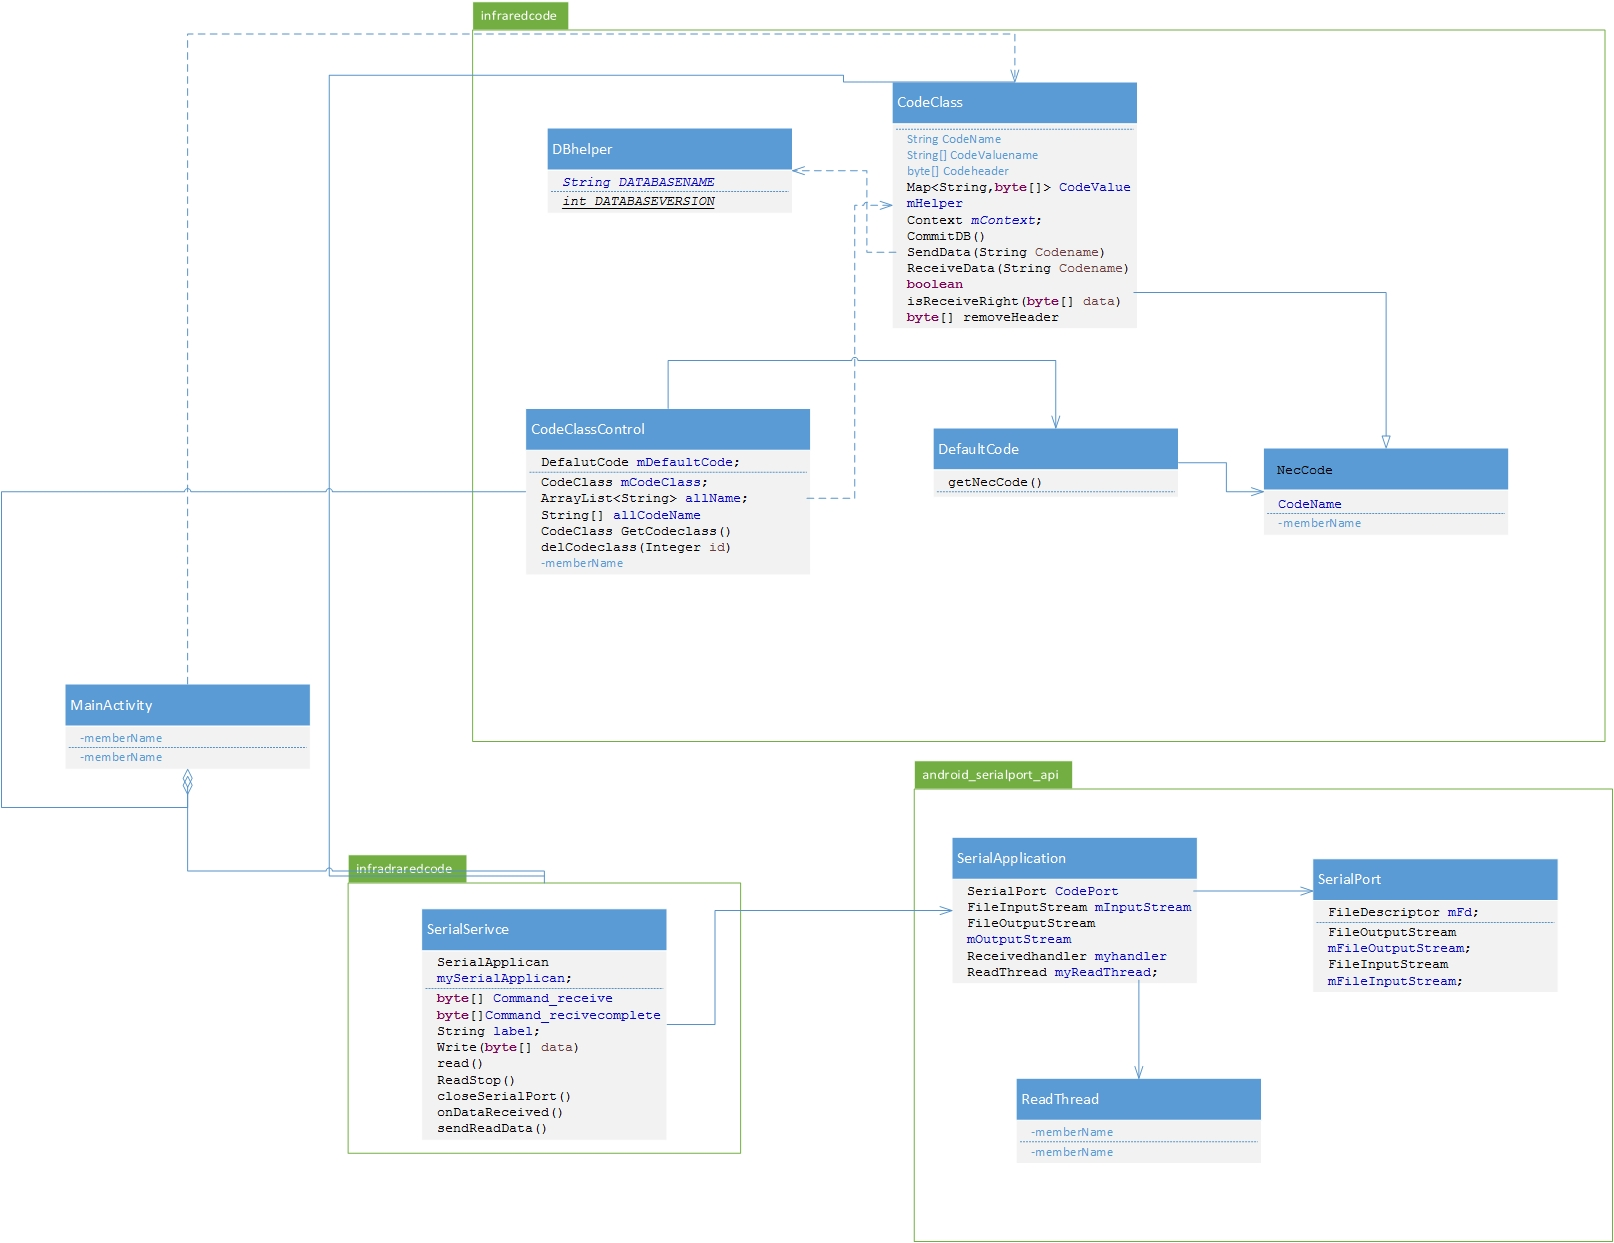
\includegraphics{Class.jpg}

There are a few things to note
\begin{enumerate}
\item {} 
This app runs successfully in the android Development Board which mode is Intel Sharks Cove. So theoretically It can be compatible with all x86 and arm cpu.

\item {} 
This app need root permission.

\end{enumerate}


\section{Work flow}
\label{base:work-flow}\phantomsection\label{base:tutorialr}
this is the APP‘s MainActivity initialization process.If you want to modify this App deeply, you can refer to this process , if you just want to add some special button, or change the layout ,We recommend that you refer to the second {\color{red}\bfseries{}tutorial\_}.

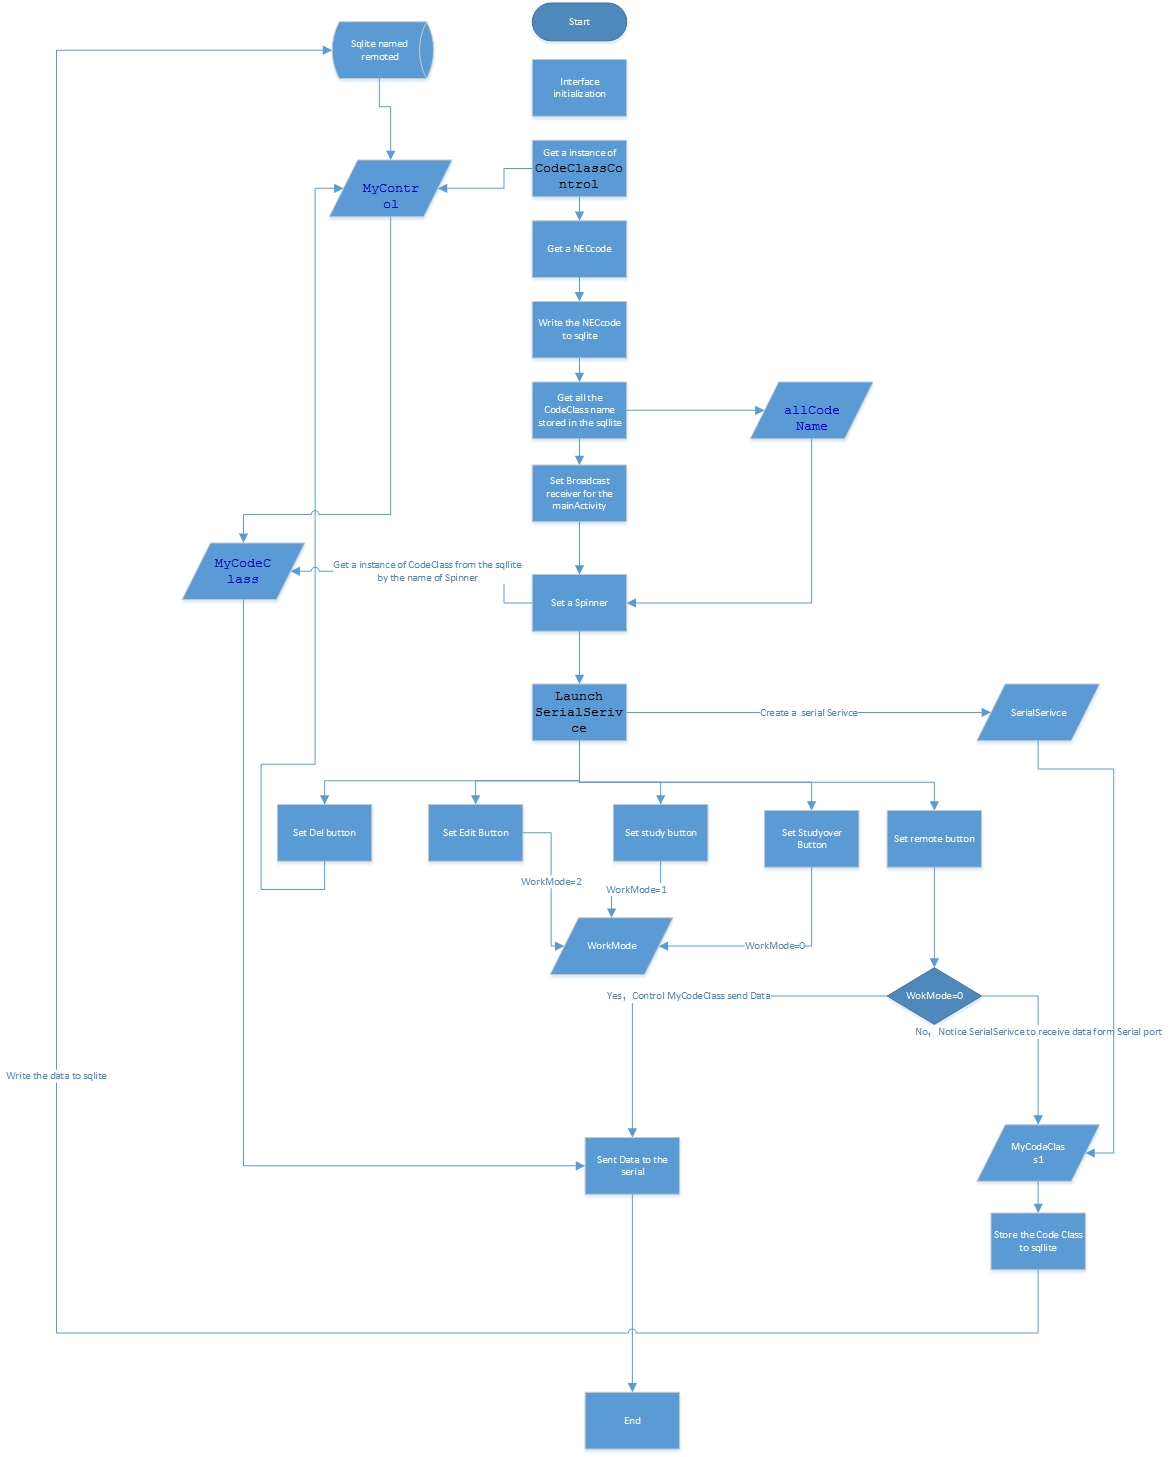
\includegraphics{workflow.jpg}


\chapter{This is a introduction of how to  extend the app (add button)}
\label{extension::doc}\label{extension:this-is-a-introduction-of-how-to-extend-the-app-add-button}
The remote Android App  is a complement  demo of cms' FPGA remote IR Remote Controller.It's extensible and convenient. User can directly use it for  most scenes, but we also  provide APIs for user to develope some special remote or just use Android device‘s UART.
this page will show you the Processes and considerations when you extend this app.


\section{client.xml}
\label{extension:client-xml}
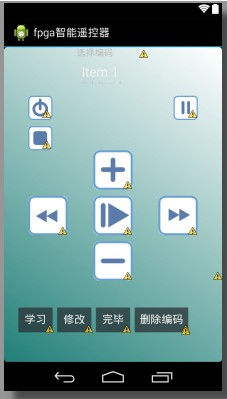
\includegraphics{interface.jpg}
\begin{enumerate}
\item {} 
This is the \emph{remote button code} part,you can add your remote button among them. we recommand adding \emph{imagebutton} which will auto include click effects.

\end{enumerate}

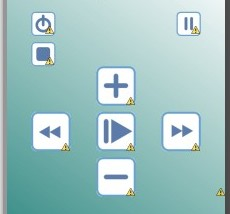
\includegraphics{remotebutton.jpg}

\begin{Verbatim}[commandchars=\\\{\}]
 \PYG{n+nt}{\PYGZlt{}RelativeLayout}
    \PYG{n+na}{android:layout\PYGZus{}width=}\PYG{l+s}{\PYGZdq{}fill\PYGZus{}parent\PYGZdq{}}
    \PYG{n+na}{android:layout\PYGZus{}height=}\PYG{l+s}{\PYGZdq{}wrap\PYGZus{}content\PYGZdq{}}
    \PYG{n+na}{android:id=}\PYG{l+s}{\PYGZdq{}@+id/buttonfield\PYGZdq{}}\PYG{n+nt}{\PYGZgt{}}\PYGZdq{}
    \PYG{n+nt}{\PYGZlt{}ImageButton}
        \PYG{n+na}{android:id=}\PYG{l+s}{\PYGZdq{}@+id/power\PYGZdq{}}
        \PYG{n+na}{android:layout\PYGZus{}width=}\PYG{l+s}{\PYGZdq{}40dip\PYGZdq{}}
        \PYG{n+na}{android:layout\PYGZus{}height=}\PYG{l+s}{\PYGZdq{}40dip\PYGZdq{}}
        \PYG{n+na}{android:layout\PYGZus{}alignParentLeft=}\PYG{l+s}{\PYGZdq{}true\PYGZdq{}}
        \PYG{n+na}{android:layout\PYGZus{}alignParentTop=}\PYG{l+s}{\PYGZdq{}true\PYGZdq{}}
        \PYG{n+na}{android:layout\PYGZus{}marginLeft=}\PYG{l+s}{\PYGZdq{}40dip\PYGZdq{}}
        \PYG{n+na}{android:layout\PYGZus{}marginTop=}\PYG{l+s}{\PYGZdq{}20dip\PYGZdq{}}
        \PYG{n+na}{android:background=}\PYG{l+s}{\PYGZdq{}@drawable/power\PYGZdq{}} \PYG{n+nt}{/\PYGZgt{}}
    \PYG{n+nt}{\PYGZlt{}ImageButton}
        \PYG{n+na}{android:id=}\PYG{l+s}{\PYGZdq{}@+id/cli1\PYGZdq{}}
        \PYG{n+na}{android:layout\PYGZus{}width=}\PYG{l+s}{\PYGZdq{}40dip\PYGZdq{}}
        \PYG{n+na}{android:layout\PYGZus{}height=}\PYG{l+s}{\PYGZdq{}40dip\PYGZdq{}}
        \PYG{n+na}{android:layout\PYGZus{}alignParentLeft=}\PYG{l+s}{\PYGZdq{}true\PYGZdq{}}
        \PYG{n+na}{android:layout\PYGZus{}below=}\PYG{l+s}{\PYGZdq{}@+id/power\PYGZdq{}}
        \PYG{n+na}{android:layout\PYGZus{}marginLeft=}\PYG{l+s}{\PYGZdq{}40dip\PYGZdq{}}
        \PYG{n+na}{android:layout\PYGZus{}marginTop=}\PYG{l+s}{\PYGZdq{}10dip\PYGZdq{}}
        \PYG{n+na}{android:background=}\PYG{l+s}{\PYGZdq{}@drawable/cli1\PYGZdq{}} \PYG{n+nt}{/\PYGZgt{}}
    \PYG{n+nt}{\PYGZlt{}ImageButton}
        \PYG{n+na}{android:id=}\PYG{l+s}{\PYGZdq{}@+id/cli2\PYGZdq{}}
        \PYG{n+na}{android:layout\PYGZus{}width=}\PYG{l+s}{\PYGZdq{}40dip\PYGZdq{}}
        \PYG{n+na}{android:layout\PYGZus{}height=}\PYG{l+s}{\PYGZdq{}40dip\PYGZdq{}}
        \PYG{n+na}{android:layout\PYGZus{}alignParentRight=}\PYG{l+s}{\PYGZdq{}true\PYGZdq{}}
        \PYG{n+na}{android:layout\PYGZus{}alignTop=}\PYG{l+s}{\PYGZdq{}@+id/power\PYGZdq{}}
        \PYG{n+na}{android:layout\PYGZus{}marginRight=}\PYG{l+s}{\PYGZdq{}40dip\PYGZdq{}}
        \PYG{n+na}{android:background=}\PYG{l+s}{\PYGZdq{}@drawable/cli2\PYGZdq{}} \PYG{n+nt}{/\PYGZgt{}}

    \PYG{n+nt}{\PYGZlt{}ImageButton}
        \PYG{n+na}{android:id=}\PYG{l+s}{\PYGZdq{}@+id/volume\PYGZus{}add\PYGZdq{}}
        \PYG{n+na}{android:layout\PYGZus{}width=}\PYG{l+s}{\PYGZdq{}65dip\PYGZdq{}}
        \PYG{n+na}{android:layout\PYGZus{}height=}\PYG{l+s}{\PYGZdq{}65dip\PYGZdq{}}
        \PYG{n+na}{android:layout\PYGZus{}below=}\PYG{l+s}{\PYGZdq{}@+id/cli1\PYGZdq{}}
        \PYG{n+na}{android:layout\PYGZus{}centerHorizontal=}\PYG{l+s}{\PYGZdq{}true\PYGZdq{}}
        \PYG{n+na}{android:background=}\PYG{l+s}{\PYGZdq{}@drawable/valume\PYGZus{}add\PYGZdq{}} \PYG{n+nt}{/\PYGZgt{}}

    \PYG{n+nt}{\PYGZlt{}ImageButton}
        \PYG{n+na}{android:id=}\PYG{l+s}{\PYGZdq{}@+id/play\PYGZdq{}}
        \PYG{n+na}{android:layout\PYGZus{}width=}\PYG{l+s}{\PYGZdq{}65dip\PYGZdq{}}
        \PYG{n+na}{android:layout\PYGZus{}height=}\PYG{l+s}{\PYGZdq{}65dip\PYGZdq{}}
        \PYG{n+na}{android:layout\PYGZus{}alignLeft=}\PYG{l+s}{\PYGZdq{}@+id/volup\PYGZdq{}}
        \PYG{n+na}{android:layout\PYGZus{}below=}\PYG{l+s}{\PYGZdq{}@+id/volume\PYGZus{}add\PYGZdq{}}
        \PYG{n+na}{android:layout\PYGZus{}centerInParent=}\PYG{l+s}{\PYGZdq{}true\PYGZdq{}}
        \PYG{n+na}{android:layout\PYGZus{}marginTop=}\PYG{l+s}{\PYGZdq{}10dip\PYGZdq{}}
        \PYG{n+na}{android:background=}\PYG{l+s}{\PYGZdq{}@drawable/center\PYGZdq{}} \PYG{n+nt}{/\PYGZgt{}}

    \PYG{n+nt}{\PYGZlt{}ImageButton}
        \PYG{n+na}{android:id=}\PYG{l+s}{\PYGZdq{}@+id/prev\PYGZdq{}}
        \PYG{n+na}{android:layout\PYGZus{}width=}\PYG{l+s}{\PYGZdq{}65dip\PYGZdq{}}
        \PYG{n+na}{android:layout\PYGZus{}height=}\PYG{l+s}{\PYGZdq{}65dip\PYGZdq{}}
        \PYG{n+na}{android:layout\PYGZus{}alignLeft=}\PYG{l+s}{\PYGZdq{}@+id/cli1\PYGZdq{}}
        \PYG{n+na}{android:layout\PYGZus{}alignTop=}\PYG{l+s}{\PYGZdq{}@+id/play\PYGZdq{}}
        \PYG{n+na}{android:layout\PYGZus{}below=}\PYG{l+s}{\PYGZdq{}@+id/volume\PYGZus{}add\PYGZdq{}}
        \PYG{n+na}{android:background=}\PYG{l+s}{\PYGZdq{}@drawable/prev\PYGZdq{}} \PYG{n+nt}{/\PYGZgt{}}

    \PYG{n+nt}{\PYGZlt{}ImageButton}
        \PYG{n+na}{android:id=}\PYG{l+s}{\PYGZdq{}@+id/next\PYGZdq{}}
        \PYG{n+na}{android:layout\PYGZus{}width=}\PYG{l+s}{\PYGZdq{}65dip\PYGZdq{}}
        \PYG{n+na}{android:layout\PYGZus{}height=}\PYG{l+s}{\PYGZdq{}65dip\PYGZdq{}}
        \PYG{n+na}{android:layout\PYGZus{}alignRight=}\PYG{l+s}{\PYGZdq{}@+id/cli2\PYGZdq{}}
        \PYG{n+na}{android:layout\PYGZus{}alignTop=}\PYG{l+s}{\PYGZdq{}@+id/play\PYGZdq{}}
        \PYG{n+na}{android:background=}\PYG{l+s}{\PYGZdq{}@drawable/next\PYGZdq{}} \PYG{n+nt}{/\PYGZgt{}}

    \PYG{n+nt}{\PYGZlt{}ImageButton}
        \PYG{n+na}{android:id=}\PYG{l+s}{\PYGZdq{}@+id/volume\PYGZus{}down\PYGZdq{}}
        \PYG{n+na}{android:layout\PYGZus{}width=}\PYG{l+s}{\PYGZdq{}65dip\PYGZdq{}}
        \PYG{n+na}{android:layout\PYGZus{}height=}\PYG{l+s}{\PYGZdq{}65dip\PYGZdq{}}
        \PYG{n+na}{android:layout\PYGZus{}alignLeft=}\PYG{l+s}{\PYGZdq{}@+id/play\PYGZdq{}}
        \PYG{n+na}{android:layout\PYGZus{}below=}\PYG{l+s}{\PYGZdq{}@+id/play\PYGZdq{}}
        \PYG{n+na}{android:layout\PYGZus{}marginTop=}\PYG{l+s}{\PYGZdq{}10dip\PYGZdq{}}
        \PYG{n+na}{android:background=}\PYG{l+s}{\PYGZdq{}@drawable/volume\PYGZus{}down\PYGZdq{}} \PYG{n+nt}{/\PYGZgt{}}
\PYG{n+nt}{\PYGZlt{}/RelativeLayout\PYGZgt{}}
\end{Verbatim}
\begin{enumerate}
\setcounter{enumi}{1}
\item {} 
This is the \emph{command button code} part. We do not recommend changing this part.

\end{enumerate}

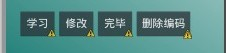
\includegraphics{command.jpg}

\begin{Verbatim}[commandchars=\\\{\}]
  \PYG{n+nt}{\PYGZlt{}RelativeLayout}
    \PYG{n+na}{android:id=}\PYG{l+s}{\PYGZdq{}@+id/relate\PYGZus{}level1\PYGZdq{}}
    \PYG{n+na}{android:layout\PYGZus{}width=}\PYG{l+s}{\PYGZdq{}wrap\PYGZus{}content\PYGZdq{}}
    \PYG{n+na}{android:layout\PYGZus{}height=}\PYG{l+s}{\PYGZdq{}50dp\PYGZdq{}}
    \PYG{n+na}{android:layout\PYGZus{}alignParentBottom=}\PYG{l+s}{\PYGZdq{}true\PYGZdq{}}
    \PYG{n+na}{android:layout\PYGZus{}centerHorizontal=}\PYG{l+s}{\PYGZdq{}true\PYGZdq{}}
    \PYG{n+na}{android:layout\PYGZus{}marginTop=}\PYG{l+s}{\PYGZdq{}40dp\PYGZdq{}}\PYG{n+nt}{\PYGZgt{}}
 \PYG{n+nt}{\PYGZlt{}Button}
     \PYG{n+na}{android:layout\PYGZus{}width=}\PYG{l+s}{\PYGZdq{}wrap\PYGZus{}content\PYGZdq{}}
      \PYG{n+na}{android:layout\PYGZus{}height=}\PYG{l+s}{\PYGZdq{}wrap\PYGZus{}content\PYGZdq{}}
      \PYG{n+na}{android:layout\PYGZus{}marginLeft=}\PYG{l+s}{\PYGZdq{}20dp\PYGZdq{}}
      \PYG{n+na}{android:id=}\PYG{l+s}{\PYGZdq{}@+id/study\PYGZdq{}}
     \PYG{n+na}{android:text=}\PYG{l+s}{\PYGZdq{}学习\PYGZdq{}}\PYG{n+nt}{/\PYGZgt{}}
 \PYG{n+nt}{\PYGZlt{}Button}
     \PYG{n+na}{android:layout\PYGZus{}width=}\PYG{l+s}{\PYGZdq{}wrap\PYGZus{}content\PYGZdq{}}
      \PYG{n+na}{android:layout\PYGZus{}height=}\PYG{l+s}{\PYGZdq{}wrap\PYGZus{}content\PYGZdq{}}
      \PYG{n+na}{android:layout\PYGZus{}toRightOf=}\PYG{l+s}{\PYGZdq{}@id/study\PYGZdq{}}
      \PYG{n+na}{android:id=}\PYG{l+s}{\PYGZdq{}@+id/edit\PYGZdq{}}
     \PYG{n+na}{android:text=}\PYG{l+s}{\PYGZdq{}修改\PYGZdq{}}\PYG{n+nt}{/\PYGZgt{}}
  \PYG{n+nt}{\PYGZlt{}Button}
     \PYG{n+na}{android:layout\PYGZus{}width=}\PYG{l+s}{\PYGZdq{}wrap\PYGZus{}content\PYGZdq{}}
      \PYG{n+na}{android:layout\PYGZus{}height=}\PYG{l+s}{\PYGZdq{}wrap\PYGZus{}content\PYGZdq{}}
      \PYG{n+na}{android:layout\PYGZus{}toRightOf=}\PYG{l+s}{\PYGZdq{}@id/edit\PYGZdq{}}
      \PYG{n+na}{android:id=}\PYG{l+s}{\PYGZdq{}@+id/studyover\PYGZdq{}}
     \PYG{n+na}{android:text=}\PYG{l+s}{\PYGZdq{}完毕\PYGZdq{}}\PYG{n+nt}{/\PYGZgt{}}

     \PYG{n+nt}{\PYGZlt{}Button}
         \PYG{n+na}{android:id=}\PYG{l+s}{\PYGZdq{}@+id/delete\PYGZdq{}}
         \PYG{n+na}{android:layout\PYGZus{}width=}\PYG{l+s}{\PYGZdq{}wrap\PYGZus{}content\PYGZdq{}}
         \PYG{n+na}{android:layout\PYGZus{}height=}\PYG{l+s}{\PYGZdq{}wrap\PYGZus{}content\PYGZdq{}}
         \PYG{n+na}{android:layout\PYGZus{}toRightOf=}\PYG{l+s}{\PYGZdq{}@id/studyover\PYGZdq{}}
         \PYG{n+na}{android:text=}\PYG{l+s}{\PYGZdq{}删除编码\PYGZdq{}} \PYG{n+nt}{/\PYGZgt{}}

\PYG{n+nt}{\PYGZlt{}/RelativeLayout\PYGZgt{}}
\end{Verbatim}


\section{the process of  add button}
\label{extension:the-process-of-add-button}
there are only six remote button in the demo,you can add your button conveniently, Here's an example of adding  remote button \emph{MUTE}
\begin{enumerate}
\item {} 
Add a Imagebutton in the xml, Attention: you need a button named mute in the drawer folder

\end{enumerate}

\begin{Verbatim}[commandchars=\\\{\}]
\PYG{n+nt}{\PYGZlt{}ImageButton}
             \PYG{n+na}{android:id=}\PYG{l+s}{\PYGZdq{}@+id/mute\PYGZdq{}}
             \PYG{n+na}{android:layout\PYGZus{}width=}\PYG{l+s}{\PYGZdq{}40dip\PYGZdq{}}
             \PYG{n+na}{android:layout\PYGZus{}height=}\PYG{l+s}{\PYGZdq{}40dip\PYGZdq{}}
             \PYG{n+na}{android:layout\PYGZus{}alignParentLeft=}\PYG{l+s}{\PYGZdq{}true\PYGZdq{}}
             \PYG{n+na}{android:layout\PYGZus{}below=}\PYG{l+s}{\PYGZdq{}@+id/power\PYGZdq{}}
             \PYG{n+na}{android:layout\PYGZus{}marginLeft=}\PYG{l+s}{\PYGZdq{}40dip\PYGZdq{}}
             \PYG{n+na}{android:layout\PYGZus{}marginTop=}\PYG{l+s}{\PYGZdq{}10dip\PYGZdq{}}
             \PYG{n+na}{android:background=}\PYG{l+s}{\PYGZdq{}@drawable/mute\PYGZdq{}} \PYG{n+nt}{/\PYGZgt{}}
\end{Verbatim}
\begin{enumerate}
\setcounter{enumi}{1}
\item {} 
Add a Imagebutton declaration in the Mainactivity

\end{enumerate}

\begin{Verbatim}[commandchars=\\\{\}]
\PYG{k+kd}{private} \PYG{n}{ImageButton} \PYG{n}{mute}\PYG{o}{;}
\PYG{n}{volume\PYGZus{}up}\PYG{o}{=}\PYG{o}{(}\PYG{n}{ImageButton}\PYG{o}{)}\PYG{n}{findViewById}\PYG{o}{(}\PYG{n}{R}\PYG{o}{.}\PYG{n+na}{id}\PYG{o}{.}\PYG{n+na}{mute}\PYG{o}{)}\PYG{o}{;}
\end{Verbatim}
\begin{enumerate}
\setcounter{enumi}{2}
\item {} 
Set a cliklistener for the Imagebutton

\end{enumerate}

\begin{Verbatim}[commandchars=\\\{\}]
\PYG{n}{mute}\PYG{o}{.}\PYG{n+na}{setOnClickListener}\PYG{o}{(}\PYG{k}{new} \PYG{n}{OnClickListener}\PYG{o}{(}\PYG{o}{)}\PYG{o}{\PYGZob{}}
                        \PYG{n+nd}{@Override}
                \PYG{k+kd}{public} \PYG{k+kt}{void} \PYG{n+nf}{onClick}\PYG{o}{(}\PYG{n}{View} \PYG{n}{v}\PYG{o}{)} \PYG{o}{\PYGZob{}}
                        \PYG{c+c1}{// TODO Auto\PYGZhy{}generated method stub}
                        \PYG{k}{if}\PYG{o}{(}\PYG{n}{WorkMode}\PYG{o}{=}\PYG{o}{=}\PYG{l+m+mi}{0}\PYG{o}{)}\PYG{o}{\PYGZob{}}

                                \PYG{n}{MyCodeClass}\PYG{o}{.}\PYG{n+na}{SendData}\PYG{o}{(}\PYG{l+s}{\PYGZdq{}MUTE\PYGZdq{}}\PYG{o}{)}\PYG{o}{;}
                        \PYG{o}{\PYGZcb{}}\PYG{k}{else}
                        \PYG{o}{\PYGZob{}}
                        \PYG{n}{CodeClass}\PYG{o}{.}\PYG{n+na}{ReceiveData}\PYG{o}{(}\PYG{l+s}{\PYGZdq{}MUTE\PYGZdq{}}\PYG{o}{)}\PYG{o}{;}



                        \PYG{o}{\PYGZcb{}}
                \PYG{o}{\PYGZcb{}}
 \PYG{o}{\PYGZcb{}}\PYG{o}{)}\PYG{o}{;}
\end{Verbatim}

There are a few things to Attention
\begin{enumerate}
\item {} 
You can redesign the interface  following your favorite style.

\item {} 
wo don't recommended that you change the ID of the views,becasue most of them are bound in the Mainactivity.

\end{enumerate}


\section{Waring:}
\label{extension:waring}
Currently the keywords supported by the sqllite are listed below:

``NUM1''(数字键),''NUM2'',''NUM3'',''NUM4'',''NUM5'',''NUM6'',''NUM7'',''NUM9'',''NUM0'',''PAUSE''(暂停),''LIKE''(喜爱) ,''SINALSOURCE'' (切换信号源),''SLEEP''(睡眠),''MENU'',''MUTE(静音)'', ``OK'',''POWER''(电源键),''PLAY'',''PRE'',''NEXT'',''VOLUME\_DOWN'',''VOLUME\_UP'' \};

There are a few things to Attention:
\begin{enumerate}
\item {} 
Keywords there has no capacity constraints, eg.you can learn your reality remote mute button on the ``POWER'' or other keywordes.

\item {} 
wo don't recommended that you change the ID of the views,becasue most of them are bound in the Mainactivity.

\end{enumerate}



\renewcommand{\indexname}{Index}
\printindex
\end{CJK} 
\end{document}
